\documentclass[notes.tex]{subfiles}

\graphicspath{ {images/} }

\begin{document}

\setcounter{section}{7}
\section{Additional Topics}

\subsection{Sampling from Probability Distributions}
We will first talk about how to generate samples from a probability distribution. Why is this useful? Suppose we wish to simulate a radioactive decay process on a computer. A reasonable model for the times between subsequent decays of our radioactive isotope is the exponential distribution. Thus we need to be able to generate samples from an exponential distribution. For common distributions, such as the exponential distribution, there are built-in routines in Matlab or SciPy (python) to do this. It is useful, however, to know how this works since many times the distribution you want to sample does not have a built-in routine.\\

For simplicity, we will only discuss sampling from continuous random variables. The same ideas work for discrete random variable, with a few alterations. We will also assume that we have a method for generating samples from the Uniform[0, 1] distribution. This is a very interesting problem, and there are many ways to do it, most of which are not straightforward. If you find this interesting, the topic is discussed in courses on computational probability and in some computer science courses. We will discuss two methods of sampling from probability distributions: the inverse CDF method and rejection sampling.\\

\subsubsection{Inverse CDF method}
Suppose we have a population whose distribution is characterized by a CDF $F(y)$. Recall that for a random variable $Y$, the CDF is defined as $F(y) = \P(Y \leq y)$. We would like to generate samples from the population. The inverse CDF method works as follows:
\begin{enumerate}
\item Generate $U$, a sample from the Uniform[0, 1] distribution.
\item Let $Y$ be the largest number $x$ such that $F(x) \leq u$. If the CDF $F(y)$ is \emph{strictly} increasing, then $F(y)$ is invertible so we can let $Y = F^{-1}(U)$.
\end{enumerate}
It is perhaps easier to see this on a picture. This is an example of the inverse CDF method used on a population which has a exponential distribution with parameter $\lambda = 1$.
\begin{figure}[H]
\centering
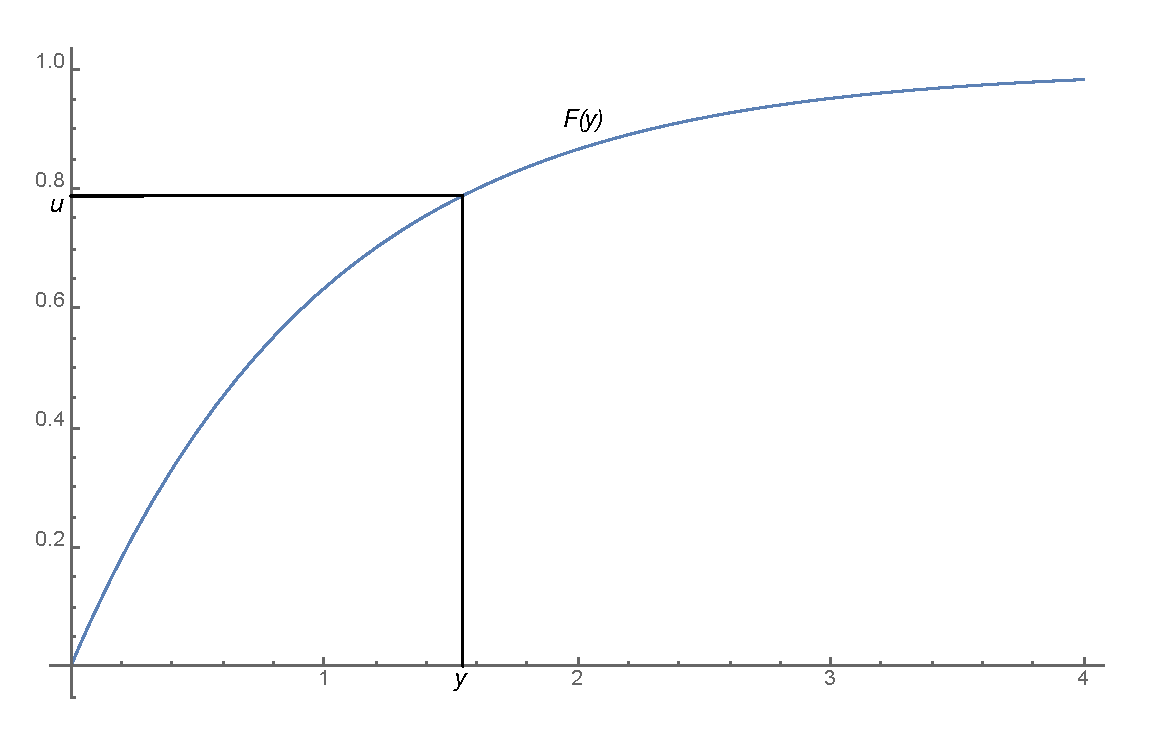
\includegraphics[width=8cm]{inversecdfexp}
\end{figure}
Why does this work. For simplicity, let's consider only the case where the CDF $F(y)$ is invertible. (Invertibility of the CDF is not required; in particular, it works for discrete random variables, whose CDF is not invertible). Let $U \sim$ Uniform[0, 1]. Then we claim the distribution of $F^{-1}(U)$ is $F$. To see this, we look at the CDF of $F^{-1}(U)$.
\begin{align*}
\P( F^{-1}(U) \leq y) &= \P(U \leq F(y) ) \\
&= F(y)
\end{align*}
where we used the fact that for a Uniform[0, 1] random variable $U$, the CDF is $\P(U \leq u) = u$ for $u \in [0, 1]$.\\

Now that we've seen the picture, let's use the inverse CDF method to sample from an exponentially distributed population.

\begin{example}Suppose we have a population which has an exponential distribution with parameter $\lambda$. Let $U$ be a Uniform[0, 1] random variable. Use the inverse CDF method to generate a sample from the population in terms of $U$.\\

First we need to find the CDF for the population. Integrating the density function from 0 to $y$:
\begin{align*}
F(y) &= \int_0^y \lambda e^{-\lambda t} dt \\
&= e^{-\lambda t}\Bigr|0^y \\
&= 1 - e^{-\lambda y}
\end{align*}
With appropriate bounds, the CDF is:
\[
F(y) = \begin{cases}
1 - e^{-\lambda y} & y \geq 0 \\
0 & \text{otherwise}
\end{cases}
\]
The CDF $F(y)$ is strictly increasing, it has an inverse. Since we want $Y = F^{-1}(U)$, we take $F(Y) = U$ and solve for $Y$.
\begin{align*}
1 - e^{-\lambda Y} &= U \\
e^{-\lambda Y} &= 1 - U \\
-\lambda Y &= \log(1 - U) \\
Y &= - \frac{1}{\lambda} \log(1 - U)
\end{align*}
\end{example}
For the exponential distribution this is very straightforward. In general this method works if we can easily compute the CDF. For continuous distributions, if the integral of the density has a nice closed form (as in the exponential case), the inverse CDF method usually works very well. For discrete distributions, this method also works well since to find the discrete CDF, all we have to do is add up the probabilities of the appropriate simple events. For cases where the CDF does not have a closed form (such as the normal distribution) or cases where the CDF is hard to invert, this method is not so good. For many of those cases, rejection sampling is the way to go.

\subsubsection{Rejection Sampling}
Rejection sampling is based on the ``dartboard principle''. Here's how it works. Imagine you have a continuous probability density function $f(x)$ you wish to sample from. Furthermore, imagine that the density function is nonzero only on the interval $[a, b]$. Put the density function on a rectangular dartboard. The bounds of the dartboard are from $a$ to $b$ in the $x$-direction and from $0$ to $M$ in the $y$-direction, where $M$ is the maximum of $f(x)$ on $[a, b]$\footnote{Recall that a continuous function has an absolute maximum on a closed interval $[a, b]$ and that density functions are nonnegative; thus this rectangular dartboard will have finite size.}. Here is an example of a possible dartboard.
\begin{figure}[H]
\centering
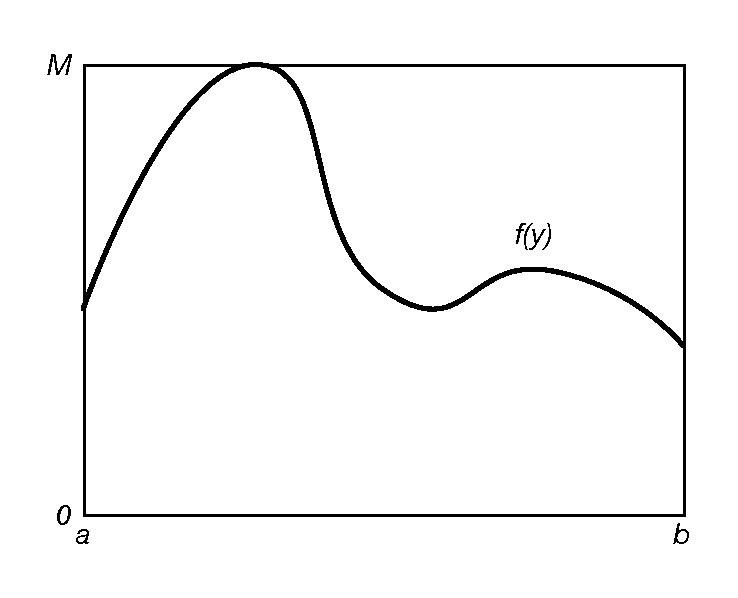
\includegraphics[width=8cm]{rejection1}
\end{figure}
Now throw darts uniformly at the dartboard until your dart lands under the density curve $f(x)$. In other words, reject all darts which do not land under the density curve (this is why we call this rejection sampling). Then your dart will be uniformly distributed in the region between the $x$-axis and the density curve, and the $x$-coordinate of your dart will be distributed according to the density $f(x)$. Intuitively, this works since there is more room on the board for (nonrejected) darts to land where the density curve is highest, i.e. where the probability density is greatest.\\

Let's show mathematically that this actually works. We have all the tools we need from the section on multivariate distributions! Let $(X, Y)$ be the position of a nonrejected dart. Then the pair $(X, Y)$ is uniformly distributed on the region between the $x$-axis and the density curve. Since we are assuming that the density $f(x)$ is zero outside $[a, b]$, the area of the region is $\int_a^b f(x) dx = 1$ since $f(x)$ is a probability density function. Since the joint density function of a uniform distribution is the reciprocal of the area of the region, for our joint density function we have joint density:
\[
f(x, y) = \begin{cases}
1 & a \leq x \leq b, 0 \leq y \leq f(x) \\
0 & \text{otherwise}
\end{cases}
\]
We claim the marginal density of $X$ is the density $f(x)$. To see this, all we have to do is integrate the joint density in $y$.
\begin{align*}
f_X(x) &= \int_0^{f(x)} 1 dy \\
&= y\Bigr|_0^{f(x)} \\
&= f(x)
\end{align*}
Thus the rejection sampling method produces works as advertised. There are a few disadvantages to the method, however. First, we need to have a bounded region for the density function. Many useful probability distributions, such as the normal distribution, are unbounded. To use rejection sampling for the standard normal distribution, for example, we have to impose artificial bounds on the density. For example, we could impose the bounds [-5, 5]. Since the probability is exceedingly low that a sample will be more than 5 standard deviations from the mean, this is not too unreasonable; it is important, however, to know that in doing this we are reducing the probability of extreme outliers to 0, which may not be what we want to do, especially if we are taking large numbers of samples. In addition, depending on the shape of the density function, we might have to throw many darts in order for one to not be rejected. This presents no problem theoretically, but might be a problem computationally. Take a look at the following picture of the standard normal density between -5 and 5.
\begin{figure}[H]
\centering
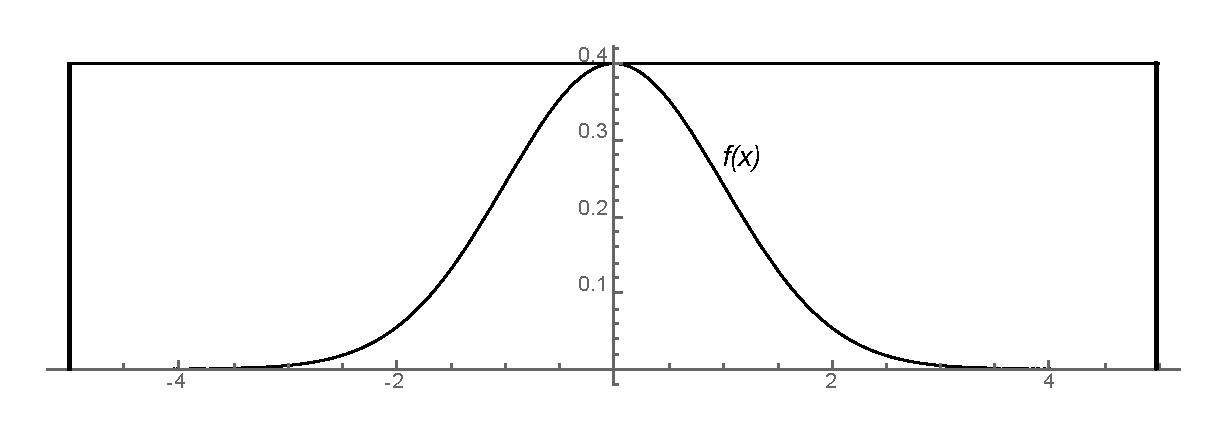
\includegraphics[width=12cm]{rejection2.eps}
\end{figure}
From the picture, the area of the rectangular dartboard is approximately 4, and the area under the curve is approximately 1, since $f(x)$ is a probability density function. Thus we expect only 1/4 of our darts to be accepted, so we will have to throw on average 4 darts to get a single sample.\\

One way around this computation inefficiency is to note that the $x$-position of our darts does not have to be uniform. In fact, it makes sense to select the $x$-position of our darts according to a density function $g(x)$ which is similar to the one we are trying to simulate and is easy to take samples from. We can think of this as throwing darts at a non-square dartboard. \\

Once again, suppose we are trying to generate a sample from a probability density function $f(x)$, where $f(x)$ is zero outside a closed interval $[a, b]$. Suppose we can generate samples from another probability density function $g(x)$, either using the inverse CDF method or some other method. The function $g(x)$ will give us the shape of our dartboard. For this to work, the function $f(x)$ must fit entirely on our dartboard. To make this happen, we scale $g(x)$ (if needed) by a constant factor $M$ so that $f(x) \leq M g(x)$ for all $x \in [a, b]$. We now throw darts uniformly at this dartboard. \\

At this point, the dartboard analogy breaks down a bit, and it is easier to just give the algorithm.
\begin{enumerate}
\item Choose $Y$ uniformly from the interval $[0,1]$.
\item Choose $X$ according to probability density $g(x)$.
\item If $Y \leq f(X) / M g(X)$, then accept the sample $(X, Y)$. $X$ is then the desired sample from the distribution $f(x)$.
\item Otherwise reject the sample and repeat from step 1.
\end{enumerate}

Mathematically, why does this work. The proof uses Bayes' theorem. Let $A$ be the event that the sample is accepted. Then by Bayes' theorem (fudging a little because density functions are not exactly probabilities but are close enough),
\begin{align*}
\P(X = x | A ) &= \frac{ \P(A | X = x) P(X = x)} {\P(A)}
\end{align*}
Since $Y$ is a uniform random variable on [0, 1],
\begin{align*}
\P(A | X = x ) &= \P \left( Y \leq \frac{ f(x) }{ M g(x) } \right) \\
&= \frac{ f(x) }{ M g(x) }
\end{align*}
where we used the density of the uniform random variable on [0, 1]. The probability $\P(X = x) = g(x)$, since $X$ is chosen according to density function $g(x)$. As mentioned above, this is not quite accurate since densities are not really probabilities, but this is good enough for our purposes. By the Law of Total Probability for continuous random variables (essentially the same as the discrete case, except we replace summation with integration),
\begin{align*}
\P(A) &= \int_a^b \P(A | X = x)\P(X = x) dx \\
&= \int_a^b \frac{f(x)}{ M g(x) } g(x) dx \\
&= \frac{1}{M} \int_a^b f(x) dx \\
&= \frac{1}{M}
\end{align*}
where we used the fact that $f(x)$ is a density function, thus integrates to 1 over the interval $[a, b]$. Thus the probability of accepting a sample is $1/M$. Putting all of this together,
\begin{align*}
\P(X = x | A ) &= \frac{ \P(A | X = x) P(X = x)} {\P(A)} \\
&= \dfrac{ \frac{f(x)}{ M g(x) } g(x) }{ \frac{1}{M} } \\
&= f(x)
\end{align*}
Thus the rejection sampling method produces a sample which is distributed according to the desired distribution $f(x)$. The probability of accepting a sample is $1 / M$. Thus if we treat the rejection sampling procedure as a sequence of Bernoulli trials with probability of success, then on average it should take $M$ trials for a sample to be accepted. (We model the number of trials needed for the first success as a geometric random variable, and use the formula for the expected value of a geometric distribution.)

\subsection{Monte Carlo Methods}

Rejection sampling is an example of a Monte Carlo method. Monte Carlo methods are a class of computational algorithms where numerical results are obtained by repeated random sampling. In rejection sampling, we sample repeatedly from a probability distribution until the sample is accepted, then the $x$-coordinate of the accepted sample is the value we seek. Let's look at Monte Carlo techniques more generally, and then apply them to numerical integration.\\

There is no standard definition of Monte Carlo methods. In general, the idea is to approximate an expected value with the sample mean of simulated random variables. Ideally, the expected value is a probability, an integral, or something else you care about. Consider a random variable $X$ having probability density function $f(x)$ defined on the interval $[a, b]$. Let $g(x)$ be a real-valued function of x. Then we can compute the expected value of $g(X)$ using the formula we learned in class in the continuous random variable section:
\[
\E(g(X)) = \int_a^b g(x) f(x) dx
\]
Now let's take a sample of $n$ random variables $X_1, \dots, X_n$ from the density $f(x)$ and compute the sample mean of $g(X_1), \dots, g(X_n)$, which we will call $\bar{g}_n$, where the subscript $n$ denotes the number of samples we took.
\[
\bar{g}_n = \frac{1}{n}\sum_{i=1}^n g(X_i)
\]
Taking the expected value of $\bar{g}$, we get:
\begin{align*}
\E(\bar{g}_n) &= \frac{1}{n}\sum_{i=1}^n \E(g(X_i))\\
&= \E(g(X))
\end{align*}
since all the $X_i$ have the same distribution. Thus $\bar{g}_n$ is an unbiased estimator for the expected value $\E(g(X))$. This is called the \emph{Monte Carlo estimator}. As long as the variance of $g(X)$ is finite\footnote{It suffices for $\E(g(X)$ to be finite, but that is beyond the scope of this course.}, then this is a consistent estimator for $g(X)$. Thus by the Law of Large Numbers, the Monte Carlo estimator $\bar{g}_n$ converges to the expected value $\E(g(X))$ in probability as $n \rightarrow \infty$.

We can use Monte Carlo techniques for numerical integration. We will give two Monte Carlo methods, the first based on a dartboard and second based on our Monte Carlo estimator which we defined above.\\

Suppose we want to integrate a function $f(x)$ from $a$ to $b$. Let's throw $n$ darts uniformly at the same rectangular dartboard we used above, and let $Y$ be the number of darts which land under the curve. Then $Y \sim$ Binomial$(n, p)$, where $p$ is the probability of a dart landing under the curve. The probability that a dart lands under the curve is the ratio of the area of the curve to the area of the rectangle, i.e.
\[
p = \dfrac{\int_a^b f(x) dx}{M(b-a)}
\]
Let $\hat{p}_n = Y/n$ be the unbiased estimator for $p$, where the subscript $n$ denotes the number of darts thrown. We know from the section on estimation that $\hat{p}_n$ is a consistent estimator for $p$, i.e. $\hat{p}_n$ converges to $p$ (in probability) as $n \rightarrow \infty$. By linearity,
\[
M(b-a) \hat{p}_n = M(b-a)\frac{Y}{n}
\] 
is an unbiased estimator for $\int_a^b f(x) dx$ and converges to $\int_a^b f(x) dx$ in probability as $n \rightarrow \infty$. Thus we can estimate the integral by $M(b-a)\frac{Y}{n}$. It is easy to compute this, since all we have to do is generate uniform points in the rectangle and verify that the $y$-coordinate lies under the curve.\\

Just as we did above in the case of sampling from probability distributions, Monte Carlo integration does not require that samples be chosen uniformly in a rectangle, i.e. we don't have to use a ``dartboard'' to do it. Why might it be useful to use a different approach? Suppose we want to integrate the standard normal density function from -5 to 5. If we enclose that in a rectangular dartboard and throw darts uniformly at random, many of the darts will lie in the region of the tails of the normal distribution where there is very little area. It makes sense that for a good estimate of the are under the curve, darts thrown near the center ``matter'' more than darts thrown to the edges since there is more area there. Thus it might be a good idea to throw darts whose $x$-coordinate distributed such that more darts hit the center than the edges of the dartboard. This idea is called \emph{importance sampling}. The algorithm is based on our Monte Carlo Estimator for expected values.\\

Let $f(x)$ be a continuous function, and suppose we want to estimate the integral $\int_a^b f(x) dx$. Let $g(x)$ be any probability density function defined on $[a, b]$. Take $n$ independent samples $X_1, \dots, X_n$ using the density $g(x)$ (this can be done with inverse CDF, rejection sampling, or any other method). Then the following is an unbiased estimator for $\int_a^b f(x) dx$:
\[
\hat{I}_n = \frac{1}{n}\sum_{i=1}^n \frac{ f(X_i) }{g(X_i) }
\]
What is the expected value of this estimator? Since the $X_i$ are distributed according to $g(x)$, using linearity of expectation and the formula for the expected value of a function of a random variable,
\begin{align*}
\E( \hat{I}_n ) &= \frac{1}{n} \sum_{i=1}^n \E \left( \frac{ f(X_i) }{g(X_i) }\right) \\
&= \frac{1}{n}\sum_{i=1}^n \int_a^b \frac{ f(x) }{g(x) } g(x) dx \\
&= \frac{1}{n}\sum_{i=1}^n \int_a^b f(x) dx \\
&= \int_a^b f(x) dx
\end{align*}
Thus $\hat{I}_n$ is unbiased. By the Law of Large Numbers, as $n \rightarrow \infty$, the estimator $\hat{I}_n$ converges to the integral $\int_a^b f(x) dx$ (in probability). Thus $\hat{I}_n$ is a consistent estimator for the integral $\int_a^b f(x) dx$.

\subsection{Linear Regression}

Linear regression is one of the mathematical methods most often used by professional statisticians. Linear regression is an inferential procedure which is used when one random variable $Y$, called the dependent variable, has a mean which is a function of one or more nonrandom variables $x_1, \dots, x_n$, called the independent variables. (The names ``dependent'' and ``independent'' are used in the scientific sense to indicate the roles the variables play, and do not imply anything about independence in the probabilistic sense.) What are some examples of this? 
\begin{enumerate}
\item $Y$ is the stopping distance for an automobile of a particular make and model. $Y$ is a random variable, but its mean depends on the velocity $x$ of the car before the brakes are applied.
\item $Y$ is the elongation of a strip of metal subject to a stretching force. $Y$ is a random variable whose mean depends on the applied force $x_1$ and the temperature $x_2$.
\item $Y$ is the sale price of homes in a certain neighborhood over the past month. $Y$ is a random variable whose mean depends, among other things, on $x$, the size of the home in square feet. 
\end{enumerate}

In this section we will only consider a single independent variable $x$. Consider a scatter-plot of $n$ samples of the random variable $Y$ corresponding to $n$ values of the independent variable $x$. We could, for example, plot home prices in a certain neighborhood versus the size of the home. Intuitively, you would expect that $Y$ would roughly increase as $x$ increases, since bigger homes are more likely to sell for more. A purely deterministic, linear model, which we can write as
\[
Y = \beta_0 + \beta_1 x
\]
cannot possibly fit the data, because that would imply that all the points lie exactly on a straight line. Instead, we will use a probabilistic model which says that the data lies along a straight line, but that there is random error involved so that the points do not lie exactly along the line. This model would look like:
\[
Y = \beta_0 + \beta_1 x + \epsilon
\]
where $\epsilon$ is a random variable modeling the error in the problem. The distribution of $\epsilon$ is unknown, but we will take it to have mean 0 and variance $\sigma_2$. It is often useful (and in many cases quite accurate) to take $\epsilon$ to have a normal distribution. Since $\E(\epsilon) = 0$, the expected value of $Y$ is
\[
\E(Y) = \beta_0 + \beta_1 x
\]
since everything other than $\epsilon$ is a constant. Thus, although $Y$ itself does not fall on a straight line, its expected value does. \\

A \emph{linear statistical model} models the expected value $\E(Y)$ as a linear function of one or more unknown parameters $\beta_0, \beta_1, \dots, \beta_n$. Note that the word \emph{linear} refers to the fact that $\E(Y)$ is a linear function of the parameters $\beta_i$. $\E(Y)$ is not necessarily a linear function of the independent variables. If we like, to make this clear we could write the model as $\E(Y) = x \beta_1 + \beta_0$, to show that the independent variable plays the role of the coefficient here. We shall consider here only \emph{simple linear regression} models, ones in which $\E(Y)$ is a linear function of only two unknown parameters $\beta_0$ and $\beta_1$. The following are all examples of simple linear regression models:
\begin{align*}
\E(Y) &= \beta_0 + \beta_1 x \\
\E(Y) &= \beta_0 + \beta_1 x^2 \\
\E(Y) &= \beta_0 + \beta_1 \sqrt{x} \\
\E(Y) &= \beta_0 + \beta_1 \log(x)
\end{align*}
In all the above cases, $\E(Y)$ is a linear function of the unknown parameters. The thing involving the independent variable $x$ is merely the coefficient of $\beta_1$. We can do whatever we want (take a power, root, log, exponential, etc) to the independent variable $x$ since its values are always known. A \emph{multiple linear regression model} is still a linear function of unknown parameters, but we have more than two unknown parameters. The following are examples of multiple linear regression models with three unknown parameters:
\begin{align*}
\E(Y) &= \beta_0 + \beta_1 x_1 + \beta_2 x^2 \\
\E(Y) &= \beta_0 + \beta_1 x + \beta_2 x^2
\end{align*}
Recall that the independent variables are the coefficients of the linear model. In the first case, the coefficients are $x$ and $x^2$, which are two powers of the same independent variable. In the second case, the coefficients are two different independent variables. We will only concern ourselves with simple linear regression models here.\\

The parameters $\beta_0$ and $\beta_1$ are population parameters which are unknown. We will use the method of least squares to estimate these parameters. Roughly, this is what we are doing. $Y$ represents a measurement from a population whose distribution is unknown, but whose expected value depends on an independent, nonrandom variable $x$ via a simple linear regression relationship $\E(Y) = \beta_0 + \beta_1 x$ with unknown parameters $\beta_0$ and $\beta_1$. We will estimate $\beta_0$ and $\beta_1$ in the following way. Take $n$ samples $Y_1, \dots, Y_n$ from the population, along with their corresponding values of $x_1, \dots, x_n$. In our real estate example, we select $n$ homes. Their sale price corresponds to the $Y_i$, and their size corresponds to the $x_i$. In the automobile braking example, we select $n$ different velocities $x_i$ and measure the braking distance $Y_i$ corresponding to each one. In all cases, we have $n$ ordered pairs $(x_i, Y_i)$. Plot these on a graph, and draw the ``best-fit'' straight line (you can just eyeball this!) The $y$-intercept and slope of this ``best-fit'' line are our estimators $\hat{\beta}_0$ and $\hat{\beta}_1$ for the population parameters $\beta_0$ and $\beta_1$. \\

Our estimator for the unknown parameters is nothing more than the ``best-fit'' line, which we are familiar with from high school science class! Since we want to quantify how good the estimators are, the ``eyeball method'' is not good enough. We need a method to mathematically construct the best-fit straight line through a set of points. This method is known as the \emph{method of least squares}, and is the method used by Microsoft Excel and other software packages to do this.

\subsubsection{Method of Least Squares}
Suppose we have $n$ points $(x_i, y_i)$, and we wish to fit the best possible straight line to them. Since this is an estimator, we will denote the best possible straight line by
\[
\hat{y} = \hat{\beta}_0 + \hat{\beta}_1 x
\]
In the ``eyeball method'', we want to make the line as close as possible to all the points. Mathematically, here's what we do. The $x$-value $x_i$ corresponds to the observed $y$-value $y_i$. If we plug $x_i$ into our linear model, we get our estimated $y$-value:
\[
\hat{y}_i = \hat{\beta}_0 + \hat{\beta}_1 x_i
\]
For $x_i$, the deviation of the observed value from the estimated value, called the \emph{error}, is $y_i - \hat{y}_i$. We want to minimize the \emph{sum of square errors} (SSE) of the $n$ samples. That is, we want to find the values of $\hat{\beta}_0$ and $\hat{\beta}_1$ that minimize:
\[
SSE = \sum_{i=0}^n (y_i - \hat{y}_i)^2 = \sum_{i=0}^n \left[ y_i - (\hat{\beta}_0 + \hat{\beta}_1 x_i) \right]^2 
\]
To do this requires multivariable calculus. (We could also do the minimization numerically, using the method of gradient descent). Essentially, we take the partial derivatives with respect to both $\hat{\beta}_0$ and $\hat{\beta}_1$, set them equal to 0, and solve the resulting equations for the two parameters. The algebra is lengthy and so the details will be omitted; if you like you can work through them or look up the calculations in any book on statistics. The result is presented in the box below.

\begin{framed}
  \emph{Least Squares Estimators for Simple Linear Regression }\\
  \rule{\dimexpr\linewidth-2\fboxsep-2\fboxrule}{.1pt} \\
Suppose that a random variable $Y$ and a nonrandom variable $x$ are related by a linear regression model:
\[
\E(Y) = \beta_0 + \beta_1 x
\]
Take $n$ samples $(x_1, y_1), \dots, (x_n, y_n)$. Then the least squares estimators of the parameters $\beta_0$ and $\beta_1$ are
\begin{align*}
\hat{\beta}_1 &= \dfrac{S_{xy}}{S_{xx}}\\
\hat{\beta}_0 &= \bar{y} - \hat{\beta}_1 \bar{x}
\end{align*}
where $\bar{x}$ and $\bar{y}$ are the sample means of the two variables, and
\begin{align*}
S_{xy} &= \sum_{i=1}^n (x_i - \bar{x})(y_i - \bar{y}) \\
S_{xx} &= \sum_{i=1}^n (x_i - \bar{x})^2
\end{align*}
\end{framed}

Calculating these estimators is sufficiently annoying that it should only be done on a computer! If you have studied linear algebra, there is actually a nice form for these involving matrix multiplication. Instead of doing an example (by hand) of a least squares regression, we will instead discuss properties of these estimators such as bias and variance.

\subsubsection{Properties of Least Squares Estimators}

Recall the model that we are using for simple linear regression. $Y$ is a random variable whose value depends on an independent variable $x$ with a degree of error given by $\epsilon$.
\[
Y = \beta_0 + \beta_1 x + \epsilon
\]
The error $\epsilon$ has mean 0 and variance $\sigma^2$. In particular, we assume that the variance of the error does not depend on the independent variable $x$. Thus the expected value of $Y$ is a linear function of $x$:
\[
\E(Y) = \beta_0 + \beta_1 x
\]
We will show that the least squares estimators $\hat{\beta}_0$ and $\hat{\beta}_1$ are unbiased estimators of the parameters $\beta_0$ and $\beta_1$. To form our estimators, recall that we took $n$ samples $Y_1, \dots, Y_n$ from the population. To each sample we have a corresponding value for the independent variable $x_1, \dots, x_n$. The dependent variable $Y_i$ and the independent variable $x_i$ are related according to our model:
\[
Y_i = \beta_0 + \beta_1 x_i + \epsilon_i
\]
where $\epsilon_i$ is the value of the error for the $i$th sample $(x_i, Y_i)$. The errors $\epsilon_i$ are independent and have the same distribution as $\epsilon$. Since the expected value of $\epsilon_i$ is 0, note that
\[
\E(Y_i) = \beta_0 + \beta_1 x_i
\]
Since $\beta_0 + \beta_1 x_i$ is a constant and thus adding it does not affect variance, the variance of $Y_i$ is given by
\[
Var(Y_i) = Var(\epsilon_i) = \sigma^2
\]
First let's find the bias of $\hat{\beta}_1$. We can simplify the expression for $\hat{\beta}_1$ as follows\footnote{Since all sums are from 1 to $n$, we will omit the indexes on the sum for simplicity.}:
\begin{align*}
\hat{\beta}_1 &= \dfrac{S_{xy}}{S_{xx}} \\
&= \dfrac{ \sum (x_i - \bar{x})(Y_i - \bar{Y}) }{S_{xx}} \\
&= \dfrac{ \sum (x_i - \bar{x})Y_i - \bar{Y} \sum (x_i - \bar{x}) }{S_{xx}}\\
&= \dfrac{ \sum (x_i - \bar{x})Y_i }{S_{xx}}
\end{align*}
since $\sum (x_i - \bar{x}) = n \bar{x} - n \bar{x} = 0$. Using linearity of expectation, we take the expected value of $\hat{\beta}_1$:
\begin{align*}
\E( \hat{\beta}_1 ) &= \E\left[ \dfrac{ \sum (x_i - \bar{x})Y_i }{S_{xx}} \right] \\
&= \dfrac{ \sum (x_i - \bar{x}) \E(Y_i) }{S_{xx}} \\
&= \dfrac{ \sum (x_i - \bar{x})(\beta_0 + \beta_1 x_i)}{S_{xx}} \\
&= \beta_0 \dfrac{ \sum (x_i - \bar{x})}{S_{xx}} + \beta_1 \dfrac{ \sum (x_i - \bar{x})x_i}{S_{xx}} 
\end{align*}
Note that $\sum (x_i - \bar{x}) = 0$ and 
\begin{align*}
S_{xx} &= \sum (x_i - \bar{x})^2 \\
&= \sum (x_i^2 - x_i \bar{x} - x_i \bar{x} + \bar{x}^2 ) \\
&= \sum (x_i - \bar{x})x_i - \bar{x} \sum (x_i - \bar{x}) \\
&= \sum (x_i - \bar{x})x_i 
\end{align*}
since the second sum in the second-to-last line is 0. Plugging these into the expression for the expected value of $\hat{\beta}_1$, we obtain:
\begin{align*}
\E( \hat{\beta}_1 ) &= 0 + \beta_1 \frac{ S_{xx} }{ S_{xx} } = \beta_1
\end{align*}
Thus $\hat{\beta}_1$ is an unbiased estimator for $\beta_1$. To compute its variance, we use the formula for the variance of a sum of independent random variables, together with the facts that a constant is squared when it is pulled out.
\begin{align*}
Var( \hat{\beta}_1 ) &= Var \left[ \dfrac{ \sum (x_i - \bar{x})Y_i }{S_{xx}} \right] \\
&= \frac{1}{S_{xx}^2} \sum Var \left[ (x_i - \bar{x})Y_i \right] \\
&= \frac{1}{S_{xx}^2} \sum (x_i - \bar{x})^2 Var(Y_i) 
\end{align*}
Since $Y_i = \beta_0 + \beta_1 x_i + \epsilon_i$ and the variance of $\epsilon_i$ is $\sigma^2$, $Var(Y_i) = \sigma^2$, since $\beta_0 + \beta_1 x_i$ is constant thus does not affect the variance. Putting all this together, we have:
\begin{align*}
Var( \hat{\beta}_1 ) &= \frac{1}{S_{xx}^2} \sigma^2 \sum (x_i - \bar{x})^2 \\
&= \frac{ S_{xx} }{ S_{xx}^2 } \sigma^2 \\
&= \frac{ \sigma^2 }{S_{xx}}
\end{align*}
Since $\hat{\beta}_1$ is unbiased, its mean squared error (MSE) is equal to its variance.\\

Let's do the exact same thing for the other estimator $\hat{\beta}_0$. Recall that $\hat{\beta}_0 = \bar{Y} - \hat{\beta}_1 \bar{x}$. By linearity of expectation, 
\begin{align*}
\E( \hat{\beta}_0 ) &= \E( \bar{Y} - \hat{\beta}_1 \bar{x} ) \\
&= \E( \bar{Y} ) - \bar{x} \E( \hat{\beta}_1 ) \\
&= \E( \bar{Y} ) - \beta_1 \bar{x}
\end{align*}
where we used the result from above. All we need to do is compute the expected value of $\bar{Y}$. Since our model is more complicated than in the one in the sampling distribution section (i.e. $Y$ depends on the independent random variable $x$ as well as the random error $\epsilon$), this expected value is not just the population mean. By linearity of expectation, using the expected value of $Y_i$ which we found earlier,
\begin{align*}
\E(\bar{Y}) &= \frac{1}{n} \sum \E(Y_i) \\
&= \frac{1}{n} \sum ( \beta_0 + \beta_1 x_i ) \\
&= \beta_0 + \beta_1 \frac{1}{n} \sum x_i \\
&= \beta_0 + \beta_1 \bar{x}
\end{align*}
Plugging this in above, we get:
\[
\E( \hat{\beta}_0 ) = \beta_0 + \beta_1 \bar{x} - \beta_1 \bar{x} = \beta_0
\]
Thus $\hat{\beta}_0$ is an unbiased estimator for $\beta_0$.\\

Now we find its variance. This is a little trickier since $\bar{Y}$ and $\hat{\beta_1}$ are not necessarily independent. Recalling that the general form for the variance of a sum involves the covariance,
\begin{align*}
Var(\hat{\beta}_0) &= Var( \bar{Y} - \hat{\beta}_1 \bar{x} ) \\
&= Var( \bar{Y} ) + Var( - \bar{x} \hat{\beta}_1 ) + 2 Cov (\bar{Y}, - \bar{x} \hat{\beta}_1 ) \\
&= Var( \bar{Y} ) + \bar{x}^2 Var( \hat{\beta}_1 ) - 2 \bar{x} Cov (\bar{Y}, \hat{\beta}_1 )
\end{align*}
where we used the fact that constants are squared when they are pulled out of the variance, but are pulled out without alteration from the covariance. We computed the variance of $\hat{\beta}_1$ above. Since the samples $Y_i$ are independent, the variance of $\bar{Y}$ is given by:
\begin{align*}
Var(\bar{Y}) &= \frac{1}{n^2} \sum Var(Y_i) = \frac{\sigma^2}{n}
\end{align*}
where we used the fact that $Var(Y_i) = \sigma^2$, which we derived above. Finally we compute the covariance of $\bar{Y}$ and $\hat{\beta}_1$. Here we use the fact that the covariance is linear in each argument, i.e. 
\[
Cov\left( \sum_{i=1}^n X_i, \sum_{j=1}^m Y_j\right) = \sum_{i=1}^n \sum_{j=1}^m Cov(X_i, Y_j)
\]
This can be shown using the definition of covariance or using the Magic Covariance Formula. Thus we have:
\begin{align*}
Cov (\bar{Y}, \hat{\beta}_1 ) &= Cov \left( \frac{1}{n} \sum Y_i, \frac{1}{S_{xx}}\sum (x_i - \bar{x})Y_i \right)\\
&= \frac{1}{n S_{xx} } \sum_i (x_i - \bar{x}) Cov(Y_i, Y_i) + \frac{1}{n S_{xx} } \sum_i \sum_{j \neq i} (x_j - \bar{x}) Cov(Y_i, Y_j) \\
&= \frac{1}{n S_{xx} } \sum_i (x_i - \bar{x}) Var(Y_i)
\end{align*}
since $Cov(Y_i, Y_j) = 0$ for $i \neq j$ by independence of the samples $Y_i$, and $Cov(Y_i, Y_i) = Var(Y_i)$. Since we know that the variance of $Y_i$ is $\sigma^2$, this becomes:
\begin{align*}
Cov (\bar{Y}, \hat{\beta}_1 ) &= \frac{1}{n S_{xx} } \sum_i (x_i - \bar{x}) Var(Y_i) \\
&= \frac{\sigma^2}{n S_{xx} } \sum_i (x_i - \bar{x}) = 0
\end{align*}
So the covariance of $\bar{Y}$ and $\hat{\beta_1}$ is 0, which is really convenient! Note that this does \emph{not} imply that $\bar{Y}$ and $\hat{\beta_1}$ are independent. Now we have everything we need to compute the variance of $\hat{\beta_0}$.
\begin{align*}
Var(\hat{\beta}_0) &= Var( \bar{Y} ) + \bar{x}^2 Var( \hat{\beta}_1 ) - 2 \bar{x} Cov (\bar{Y}, \hat{\beta}_1 ) \\
&= \frac{\sigma^2}{n} + \bar{x}^2 \frac{ \sigma^2 }{S_{xx}} - 0 \\
&= \sigma^2 \left( \frac{1}{n} + \frac{ \bar{x}^2 }{S_{xx}} \right) 
\end{align*}

\subsubsection{Estimation of the Variance of the Error}
The expressions for the variances of the least squares estimators are both in terms of $\sigma^2$, the variance of the error term $\epsilon$. In almost every case, this variance is unknown, thus we will use the samples themselves to estimate $\sigma^2$. Recall that if we use $\bar{Y}$ as an estimator of the population mean, we showed that the estimator
\[
\frac{1}{n-1} \sum_{i=1}^n (Y_i - \bar{Y})^2
\] 
is an unbiased estimator for the population variance. Things are little more complicated here because of the dependence on $x$. Recall that for each sample $Y_i$ we are estimating the mean $\E(Y_i)$ with the estimator
\[
\hat(Y_i) = \hat{\beta}_0 + \hat{\beta}_1 x_i
\]
Thus it seems reasonable to suppose that an estimator for the variance $\sigma^2$ of the error is based on the sum of squares error $SSE = \sum_{i=1}^n (Y_i - \hat{Y}_i)^2$. In fact, the estimator
\[
S^2 = \frac{1}{n-2} \sum_{i=1}^n (Y_i - \hat{Y}_i)^2 = \frac{1}{n-2} SSE
\]
is an unbiased estimator for $\sigma^2$. Note that the 2 in the denominator of $S^2$ is the same as the number of parameters $\beta_i$ which occur in the model. Since by linearity
\[
\E(S^2) = \frac{1}{n} \E(SSE)
\]
it suffices to find the expected value of the SSE.
\begin{align*}
\E(SSE) &= \E \left[ \sum (Y_i - \hat{Y}_i)^2 \right] \\
&= \E \left[ \sum (Y_i - \hat{\beta}_0 - \hat{\beta}_1 x_i)^2 \right] \\
&= \E \left[ \sum (Y_i - \bar{Y} + \hat{\beta}_1 \bar{x} - \hat{\beta}_1 x_i)^2 \right]
\end{align*}
where we used the fact that $\hat{\beta}_0 = \bar{Y} - \hat{\beta}_1 \bar{x}$ (this is the definition of $\hat{\beta}_0$). Thus we have:
\begin{align*}
\E(SSE) &= \E \left[ \sum [(Y_i - \bar{Y}) + \hat{\beta}_1( \bar{x} - x_i)]^2 \right]\\
&= \E\left[ \sum(Y_i - \bar{Y}) - 2 \hat{\beta}_1 \sum(Y_i - \bar{Y})( \bar{x} - x_i) + \hat{\beta}_1^2\sum( \bar{x} - x_i)^2  \right] \\
&= \E\left[ \sum(Y_i - \bar{Y}) - 2 \hat{\beta}_1 \sum(Y_i - \bar{Y})( \bar{x} - x_i) + \hat{\beta}_1^2 S_{xx} \right]
\end{align*}
Since we have:
\begin{align*}
\sum(Y_i - \bar{Y})( \bar{x} - x_i) &= S_{xy} = \hat{\beta}_1 S_{xx}
\end{align*}
and
\begin{align*}
\sum(Y_i - \bar{Y}))^2 &= \sum(Y_i^2 - 2 Y_i \bar{Y} + \bar{Y}^2 ) \\
&= \sum(Y_i)^2 - 2 \bar{Y} \sum{Y_i} + n \bar{Y}^2 \\
&= \sum(Y_i)^2 - 2 n\bar{Y}^2 + n \bar{Y}^2 \\
&= \sum(Y_i)^2 - n\bar{Y}^2 
\end{align*}
we have:
\begin{align*}
\E(SSE) &= \E \left[ \sum(Y_i)^2 - n\bar{Y}^2 - 2 \hat{\beta}_1^2 S_{xx} + \hat{\beta}_1^2 S_{xx} \right] \\
&= \E \left[ \sum(Y_i)^2 - n\bar{Y}^2 - \hat{\beta}_1^2 S_{xx} \right]\\
&= \sum \E(Y_i^2) - n \E(\bar{Y}^2) - S_{xx} \E(\hat{\beta}_1^2)
\end{align*}
We know the last term from above. For the first two terms, recall that for any random variable $X$, since $Var(X) = \E(X^2) - [\E(X)]^2$ by the Magic Variance Formula, $\E(X^2) = Var(X) + [\E(X)]^2$. Thus we have:
\begin{align*}
\E(Y_i^2) &= Var(Y_i) + [\E(Y_i)]^2 \\
&= \sigma^2 + (\beta_0 + \beta_1 x_i)^2
\end{align*}
and
\begin{align*}
\E(\bar{Y}^2) &= Var(\bar{Y}) + [\E(\bar{Y})]^2 \\
&= \frac{\sigma^2}{n} + (\beta_0 + \beta_1 \bar{x})^2
\end{align*}
and
\begin{align*}
\E(\hat{\beta_1}^2) &= Var(\hat{\beta_1}) + [\E(\hat{\beta_1})]^2 \\
&= \frac{ \sigma^2 }{S_{xx}} + \beta_1^2
\end{align*}
Plugging both of these in, we get:
\begin{align*}
\E(SSE) &= \sum (\sigma^2 + (\beta_0 + \beta_1 x_i)^2) - n \left( \frac{\sigma^2}{n} + (\beta_0 + \beta_1 \bar{x})^2 \right) - S_{xx} \left( \frac{ \sigma^2 }{S_{xx}} + \beta_1^2 \right)\\
&= n \sigma^2 + \sum (\beta_0 + \beta_1 x_i)^2 - \sigma^2 - n (\beta_0 + \beta_1 \bar{x} )^2 - \sigma^2 - \beta_1^2 S_{xx}\\
&= (n-2)\sigma^2
\end{align*}
where in the last line, everything else cancels if we expand all the squares, evaluate the sum, and simplify. Thus we conclude that $S^2$ is indeed an unbiased estimator for the variance $\sigma^2$ of the error term $\epsilon$.\\

Now that we have unbiased estimators for $\beta_0$ and $\beta_1$ and know (or know how to estimate) their variance, we can use them to construct confidence intervals and hypothesis tests for the $\beta_0$ and $\beta_1$. It is reasonable (and useful) to assume that the error $\epsilon$ is normally distributed. This is beyond the scope of this course, but these ideas (and more!) can be found in a book (or further course) on statistics.

\subsection{Bayesian Statistics}
The final topic we will discuss in this class is Bayesian statistics. We will only have time for a brief introduction, since this could be the subject of an entire course. Since Bayesian statistics is currently very popular (and since Nate Silver's election prediction methodology relies heavily on Bayesian ideas), it is worth taking a look at what it's all about.

\subsubsection{Introduction}
Bayesian statistics is a fundamentally different approach to statistics from the frequentist philosophy. In the frequentist approach, which we have used thus far in this course, we consider a population to described by a probability distribution with one or more unknown parameters. These parameters have ``true'' values which we do not know, but which we can estimate by taking samples from the population and computing estimators such as the sample mean. The more samples we take, the closer our estimate is to the ``true'' parameter value.\\

In the Bayesian approach, these population parameters do not have ``true'' values but are themselves distributed according to a probability distribution. We start with a ``best guess'' as to the distribution of the population parameter (the \emph{prior distribution}). We then take samples from our population and use Bayes' theorem to ``update'' the population distribution to obtain a \emph{posterior distribution}. We can repeat this process as many times as we want. The idea is that each time we collect more data, we learn more about the probability distribution of the parameter of interest, and \\

Let's see how this works mathematically. First, recall Bayes' theorem for two events $A$ and $B$:
\[
\P(A | B) = \frac{\P(B|A) \P(A) }{\P(B) }
\]
The denominator is typically unknown, so we can expand it using the Law of Total Probability, using any partition of the probability space. The partition $\{A, A^c\}$ is typically used, giving us the following form of Bayes' theorem.
\[
\P(A | B) = \frac{\P(B|A) \P(A) }{\P(B|A) \P(A) + \P(B|A^c) \P(A^c)}
\]
We can rewrite this as follows:
\[
\P(A | B) = \frac{1}{\P(B|A) \P(A) + \P(B|A^c) \P(A^c)} \P(B|A) \P(A)
\]
Suppose $A$ is the event we are interested in studying. The prior probability of $A$ is $\P(A)$, the probability of $A$ occurring before we know any additional information. Suppose we then observe that $B$ occurs. We are interested in updating the probability that $A$ occurs now that we know this new information. In other words, we want to know $\P(A|B)$. The term $\P(B|A)$ above is the probability that our new event $B$ occurs given $A$ occurs; this is the likelihood of $B$ given $A$. The fraction in front on the right hand side is just a constant. Thus we can write:
\[
\P(A | B) \propto \P(B|A) \P(A)
\]
This proportion captures the essence of Bayesian statistics: \emph{the posterior distribution is proportional to the product of the prior distribution and the likelihood}. Let's now rework this in terms of probability density functions and population parameters.\\

Suppose we have a population whose distribution is parameterized by $\theta$ (as before, $\theta$ could be a population mean, proportion, variance, or some other parameter). We will write then density function for the population as $f_\theta(y)$. (The population could be discrete, in which case we have a pmf $p_\theta(y)$). Since we are now Bayesian statisticians, there is no true value for $\theta$. Rather, we assume that $\theta$ is distributed according to some probability density function which we will call $g(\theta)$\footnote{This could be a pmf or a density; for the purposes of our discussion, we will assume that the population parameters are continuous random variables, so are described by a probability density function.}. \\

Now we take $n$ independent samples $Y_1, \dots, Y_n$ from the population. We form the likelihood function of our data like we have in previous sections:
\[
L(Y_1, \dots, Y_n | \theta) = \prod_{i=1}^n f_\theta(Y_i)
\]
If the population is described by a pmf $p\theta(y)$, the likelihood function is the joint probability of our data. If the population is described by a density $p\theta(y)$, the likelihood function is not quite a probability (since the probability of a point is 0), but we will treat it as if it were one. The posterior density is the conditional density of the parameter $\theta$ given our samples $Y_1, \dots, Y_n$, which we will denote:
\[
g(\theta | Y_1, \dots, Y_n)
\]
Using Bayes' theorem with these densities (pretending that densities are probabilities), we get:
\begin{align*}
g(\theta | Y_1, \dots, Y_n) &= \frac{ \P(Y_1, \dots, Y_n|\theta) g(\theta) }{ \P(Y_1, \dots, Y_n) } \\
&= \frac{ L(Y_1, \dots, Y_n|\theta) g(\theta) }{ \int L(Y_1, \dots, Y_n|\theta) g(\theta) d\theta }
\end{align*}
where the integral in the denominator is taken over all possible values of $\theta$. Since the denominator is a constant, we get the same proportionality:
\[
g(\theta | Y_1, \dots, Y_n) \propto L(Y_1, \dots, Y_n|\theta) g(\theta)
\]
In other words, the posterior density is proportional to the product of the prior density and the likelihood of the data. Let's think about how we could use this in a real-world example.

\begin{example}You are a pollster interested in the proportion $p$ of voters in Rhode Island who plan on voting for Gina Raimondo. If you were a frequentist statistician, you would take a sample of, say, 100 voters and use $\hat{p}$ the proportion of Raimondo supporters in your sample, to estimate $p$. This time, we are a Bayesian statistician. First we need to choose a prior distribution for $p$. Much of the art of Bayesian statistics involves what to choose for the prior distribution. One choice (sometimes called the naive choice) is that since we have no information at all, we could choose a Uniform[0, 1] distribution for $p$ as our prior. Now we poll voters from our population. Using the poll data and Bayes' theorem (the version above), we can update the probability distribution for $p$ using our poll data. This posterior distribution for $p$ does not give us an exact value for $p$ (it is still a probability distribution), but since it will not be uniform, it will give us a better understanding of the proportion $p$ of voters who prefer Raimondo. We can keep taking polls, updating our probability distribution for $p$ each time, to get a better and better sense of $p$ 
\end{example}

\subsubsection{Conjugate Distributions}
In some cases, there is nice relationship between the prior and the posterior distributions (this is not in general the case). This will depend on the distribution of underlying population and what is chosen for the prior distribution. For a given population distribution parameterized by $\theta$, if the posterior probability distribution $g(\theta|Y_1, \dots, Y_n)$ and the prior probability distribution $g(\theta)$ will belong to the same family, we say that the prior and posterior are \emph{conjugate distributions}. We will look at two examples of this.\\

\begin{enumerate}
\item Binomial population \\

You are a pollster interested in the proportion $p$ of voters in Rhode Island who plan on voting for Gina Raimondo. Take a sample of size $n$ from the population. Let $Y$ be the number of voters in your sample you prefer Raimondo. Then $Y \sim$ Binomial$(n, p)$. Recall the pmf for $Y$ is:
\begin{align*}
p(y) = \binom{n}{y}p^{y}(1-p)^{n-y} && y = 0, 1, \dots, n
\end{align*} 
Let's express this as a function of $p$. It takes the form
\[
g(p) = K p^a (1-p)^b
\]
where $a$ and $b$ are constants related to the distribution of $p$, and $K$ is a normalizing constant. This is not a probability distribution for $p$, but we could turn it into a probability distribution on $[0, 1]$ by choosing the normalizing constant $K$ so that $g(p)$ integrates to 1 over $[0, 1]$. The usual conjugate prior for a binomial population is the beta distribution, which is a slightly altered version of this:
\[
g(p) = \frac{ p^{\alpha - 1} (1-p)^{\beta - 1} }{ B(\alpha, \beta) }
\]
where $\alpha$ and $\beta$ are chosen to reflect your existing belief of the distribution of $p$, and $B(\alpha, \beta)$ is a normalizing constant chosen so that $g(p)$ integrates to 1 over $[0, 1]$. The values $\alpha$ and $\beta$ are called \emph{hyperparameters} of the prior distribution, to distinguish them from $p$, which is a parameter of the population. Note that in the special case where $\alpha = 1$ and $\beta = 1$, we have $g(p) = 1$, which is the uniform distribution on $[0, 1]$. If $Y$ is a beta random variable with parameters $\alpha$ and $\beta$, then the mean of $Y$ is:
\[
\E(Y) = \frac{\alpha}{\alpha + \beta}
\]

Let's use Bayes' theorem (as above) to find the posterior distribution of $p$ given our binomial data $Y$ from our $n$ samples and a prior distribution of Beta$[\alpha, \beta]$.
Bayes' theorem says that:
\[
g(p | Y) = \frac{ L(Y | p ) g(p) }{ \int L(Y|p) g(p) dp }
\] 
Note that we write our data as $Y$ instead of $Y_1, \dots, Y_n$ since $Y$ is a binomial random variable incorporating data from $n$ samples. Let's look at each of these pieces in turn. For the likelihood of the data:
\begin{align*}
L(Y | p ) = \binom{n}{Y}p^{Y}(1-p)^{n-Y}
\end{align*}
The prior distribution for $p$ is the beta distribution given above. Multiplying this by the likelihood, we get:
\begin{align*}
L(Y|p) g(p) &= \binom{n}{Y}p^{Y}(1-p)^{n-Y} \frac{ p^{\alpha - 1} (1-p)^{\beta - 1} }{ B(\alpha, \beta) }\\
&= \binom{n}{Y} \frac{1}{ B(\alpha, \beta) } p^{\alpha + Y - 1} (1-p)^{\beta + (n-Y) - 1}
\end{align*}

Putting this all together:
\begin{align*}
g(p | Y) &= \dfrac{ \binom{n}{Y} \dfrac{1}{ B(\alpha, \beta) } p^{\alpha + Y - 1} (1-p)^{\beta + (n-Y) - 1} }{ \int_0^1 \binom{n}{Y} \dfrac{1}{ B(\alpha, \beta) } p^{\alpha + Y - 1} (1-p)^{\beta + (n-Y) - 1} dp }\\
&= \dfrac{ p^{\alpha + Y - 1} (1-p)^{\beta + (n-Y) - 1} }{ \int_0^1 p^{\alpha + Y - 1} (1-p)^{\beta + (n-Y) - 1} dp }\\
&= \dfrac{ p^{\alpha + Y - 1} (1-p)^{\beta + (n-Y) - 1} }{ B(\alpha + Y - 1, \beta + (n-Y) - 1) }
\end{align*}
Where the last line follows since the denominator is the integral of the numerator, so is the normalizing constant. Comparing this to the beta density, we see that the posterior distribution is also a beta distribution, with hyperparameters $\alpha + Y$ and $\beta + (n - Y)$ (The 1s are not part of the hyperparameters; look back at the density for the beta distribution to see why this is the case). Thus we have updated our prior based on our data and obtained a posterior in the same family as the prior but with updated hyperparameters. Essentially, we have added the number of ``sucesses'' (Raimondo supporters) to $\alpha$ and the number of ``failures'' (non-Raimondo supporters) to $\beta$.\\

We can use the mean of the posterior distribution as an estimate for $p$. We call this the Bayes estimator for $p$, denoted $\hat{p}_B$. The Bayes estimator is given by:
\[
\hat{p}_B = \dfrac{ \alpha + Y }{ \alpha + Y + \beta + (n - Y) } = \dfrac{ \alpha + Y }{ \alpha + \beta + n } 
\]
We can write this estimator in a slightly different form:
\begin{align*}
\hat{p}_B &= \dfrac{ \alpha }{ \alpha + \beta + n } + \dfrac{ Y }{ \alpha + Y + \beta + (n - Y) }\\
&= \left(\dfrac{ \alpha + \beta }{ \alpha + \beta + n }\right)\dfrac{\alpha}{\alpha + \beta} + \left(\dfrac{ n }{ \alpha + \beta + n  } \right) \dfrac{Y}{n}
\end{align*}
This is a weighted average of mean of the beta prior and the sample proportion $Y/n$ (the MLE for p). The prior mean is given less weight for larger sample sizes, whereas the weight of the sample proportion increases as the sample size gets larger. Since $\E(Y/n) = p$, the Bayes estimator is not an unbiased estimator for $p$. In most cases, Bayes estimators are not unbiased.

% Let's actually try this with real polling data and see what happens. We will take the most recent polling data in Pennsylvania from \texttt{fivethirtyeight.com}. We start with a naive, uniform prior, which is a Beta[1, 1] distribution. The most recent poll I can find is Public Policy Polling (July 29-31). The number of people polled is 1505. The percentage favoring Clinton is 45\%, so the number of Clinton supporters is $1505(0.45) = 677.25$, so let's round that down to 677. The percentage favoring Trump is 42\%, so the number of Trump supporters is $1505(0.42) = 632.1$, so let's round that down to 632. Let's pretend Gary Johnson and other candidates do not exist (sorry!) so that the total number of people polled is $677 + 632 = 1309$. The the posterior distribution is Beta$[1 + 677, 1 + 632]$ = Beta$[678, 633]$. The mean is $678 / (678 + 633) = 0.517$. The graph below shows this distribution. The graph only shows the density between 0.4 and 0.6; it is essentially 0 outside this range.
% \begin{figure}[H]
% \centering
% 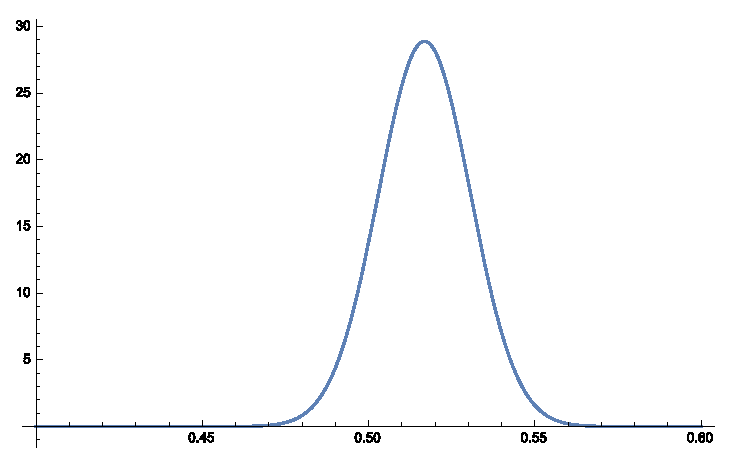
\includegraphics[width=8cm]{beta1}
% \end{figure}

\item Normal population \\

This time, suppose we have a normal population with unknown mean $\mu$ and \emph{known} variance $\sigma_0^2$. If we choose a normal distribution as a prior for the population parameter $\mu$, then the posterior distribution for $\mu$ will also be normal. Mathematically, here's how this goes.\\

Suppose we choose as our prior for the parameter $\mu$ a normal distribution with mean $\eta$ and variance $\delta^2$. That is, our prior is Normal$(\eta, \delta)$. Let $Y_1, \dots, Y_n$ be a random sample from the population, and compute the sample mean $\bar{Y}$. Then the posterior distribution for $\mu$ is also a normal distribution with mean $\eta^*$ and variance $\delta^*$ given by:
\begin{align*}
\eta^* &= \frac{\delta^2 n \bar{Y} + \sigma_0^2 \eta}{n \delta^2 + \sigma_0^2} \\
\delta^{*2} &= \frac{\sigma_0^2 \delta^2 }{n \delta^2 + \sigma_0^2}
\end{align*}
The Bayes estimator $\hat{\mu}_B$ is the mean of the normal posterior distribution. We can separate the sum in the numerator to write it as:
\[
\hat{\mu}_B = \frac{ n \delta^2 }{n \delta^2 + \sigma_0^2}\bar{Y} + \frac{\sigma_0^2}{n \delta^2 + \sigma_0^2} \eta
\]
Thus the Bayes estimator for the population mean is a weighted average of the sample mean $\bar{Y}$ (the MLE for $\mu$) and the mean of the prior $\eta$. Again, as the sample size $n$ increases, the weight given to $\bar{Y}$ increases, while the weight given to the prior mean $\eta$ decreases.
\end{enumerate}


\end{document} 